\documentclass[12pt]{report}
\usepackage[utf8]{inputenc}
\usepackage[english, russian]{babel}
\usepackage{listings}
\usepackage{graphicx}
\usepackage{float}
\graphicspath{{imgs/}}
\usepackage{amsmath,amsfonts,amssymb,amsthm,mathtools} 
\usepackage{pgfplots}
\usepackage{filecontents}
\usepackage{indentfirst}
\usepackage{eucal}
\usepackage{enumitem}
\frenchspacing

\usepackage{indentfirst} % Красная строка

\usetikzlibrary{datavisualization}
\usetikzlibrary{datavisualization.formats.functions}

\usepackage{amsmath}
\usepackage{fixltx2e}
\usepackage{caption}


\definecolor{bluekeywords}{rgb}{0,0,1}
\definecolor{greencomments}{rgb}{0,0.5,0}
\definecolor{redstrings}{rgb}{0.64,0.08,0.08}
\definecolor{xmlcomments}{rgb}{0.5,0.5,0.5}
\definecolor{types}{rgb}{0.17,0.57,0.68}

\usepackage{listings}
\lstset{language=[Sharp]C,
	captionpos=t,
	numbers=left, %Nummerierung
	numberstyle=\small, % kleine Zeilennummern
	frame=single, % Oberhalb und unterhalb des Listings ist eine Linie
	stepnumber=1,                   
	numbersep=5pt,                
	showspaces=false,
	tabsize=2,
	showtabs=false,
	breaklines=true,
	showstringspaces=false,
	breakatwhitespace=true,
	escapeinside={(*@}{@*)},
	commentstyle=\color{greencomments},
	morekeywords={partial, var, value, get, set},
	keywordstyle=\color{bluekeywords},
	stringstyle=\color{redstrings},
	basicstyle=\ttfamily\small,
}

\usepackage[left=1cm,right=1cm, top=1cm,bottom=2cm,bindingoffset=0cm]{geometry}
% Для измененных титулов глав:
\usepackage{titlesec, blindtext, color} % подключаем нужные пакеты
\definecolor{gray75}{gray}{0.75} % определяем цвет
\newcommand{\hsp}{\hspace{20pt}} % длина линии в 20pt
% titleformat определяет стиль
\titleformat{\chapter}[hang]{\Huge\bfseries}{\thechapter\hsp\textcolor{gray75}{|}\hsp}{0pt}{\Huge\bfseries}

\usepackage{array}
\newcommand{\head}[2]{\multicolumn{1}{>{\centering\arraybackslash}p{#1}}{#2}}

% plot
\usepackage{pgfplots}
\usepackage{filecontents}
\usetikzlibrary{datavisualization}
\usetikzlibrary{datavisualization.formats.functions}

\begin{document}
	%\def\chaptername{} % убирает "Глава"
	\thispagestyle{empty}
	\begin{titlepage}
		\noindent \begin{minipage}{0.15\textwidth}
			
\includegraphics[width=\linewidth]{b_logo}
		\end{minipage}
		\noindent\begin{minipage}{0.9\textwidth}\centering
			\textbf{Министерство науки и высшего образования Российской Федерации}\\
			\textbf{Федеральное государственное бюджетное образовательное учреждение высшего образования}\\
			\textbf{~~~«Московский государственный технический университет имени Н.Э.~Баумана}\\
			\textbf{(национальный исследовательский университет)»}\\
			\textbf{(МГТУ им. Н.Э.~Баумана)}
		\end{minipage}
		
		\noindent\rule{18cm}{3pt}
		\newline\newline
		\noindent ФАКУЛЬТЕТ $\underline{\text{«Информатика и системы управления»}}$ \newline\newline
		\noindent КАФЕДРА $\underline{\text{«Программное обеспечение ЭВМ и информационные технологии»}}$\newline\newline\newline\newline\newline\newline\newline\newline\newline\newline\newline
		
		
		\begin{center}
			\noindent\begin{minipage}{1.3\textwidth}\centering
				\Large\textbf{  Отчет по лабораторной работе №17-18}\newline
				\textbf{по дисциплине \newline "Функциональное и логическое программирование"}\newline\newline
			\end{minipage}
		\end{center}
		
		\noindent\textbf{Тема} $\underline{\text{Списки на Prolog}}$\newline\newline
		\noindent\textbf{Студент} $\underline{\text{Малышев И. А.}}$\newline\newline
		\noindent\textbf{Группа} $\underline{\text{ИУ7-61Б}}$\newline\newline
		\noindent\textbf{Оценка (баллы)} $\underline{\text{~~~~~~~~~~~~~~~~~~~~~~~~~~~}}$\newline\newline
		\noindent\textbf{Преподаватель: } $\underline{\text{Толпинская Н. Б.}}$\newline\newline\newline
		
		\begin{center}
			\vfill
			Москва~---~\the\year
			~г.
		\end{center}
	\end{titlepage}
	
	
	\setcounter{page}{2}

\chapter*{Лабораторная работа №17}
\section*{Задание}

Используя хвостовую рекурсию, разработать эффективную программу (комментируя назначение аргументов), позволяющую:

\begin{enumerate}
	\item Найти длину списка (по верхнему уровню);
	\item Найти сумму элементов числового списка;
	\item Найти сумму элементов числового списка, стоящих на нечетных позициях исходного списка (нумерация от 0);
\end{enumerate}

Для одного из вариантов ВОПРОСА и одного из заданий составить таблицу, отражающую конкретный порядок работы системы.

\newpage
\section*{Решение}

\begin{lstlisting}[language=prolog]
domains
	intlist = integer*

predicates
	rec_length(integer, integer, intlist)
	length(integer, intlist)
	
	rec_sum(integer, integer, intlist)
	sum(integer, intlist)
	
	rec_oddsum(integer, integer, intlist)
	oddsum(integer, intlist)

clauses
	rec_length(Res, Len, [_ | Tail]) :- NewLen = Len + 1, !, rec_length(Res, NewLen, Tail).
	rec_length(Res, Len, []) :- Res = Len.
	length(Res, List) :- rec_length(Res, 0, List).
	
	rec_sum(Res, Sum, [Head | Tail]) :- NewSum = Sum + Head, !, rec_sum(Res, NewSum, Tail).
	rec_sum(Res, Sum, []) :- Res = Sum.
	sum(Res, List) :- rec_sum(Res, 0, List).
	
	rec_oddsum(Res, Sum, [_, Head | Tail]) :- NewSum = Sum + Head, !, rec_oddsum(Res, NewSum, Tail).
	rec_oddsum(Res, Sum, []) :- Res = Sum.
	oddsum(Res, List) :- rec_oddsum(Res, 0, List).

goal
	length(Res, [1, 2, 3, 4]).
	sum(Res, [1, 2, 3, 4]).
	oddsum(Res, [1, 2, 3, 4]).
\end{lstlisting}

\section*{Порядок работы}

\begin{figure}[H]
	\begin{center}
		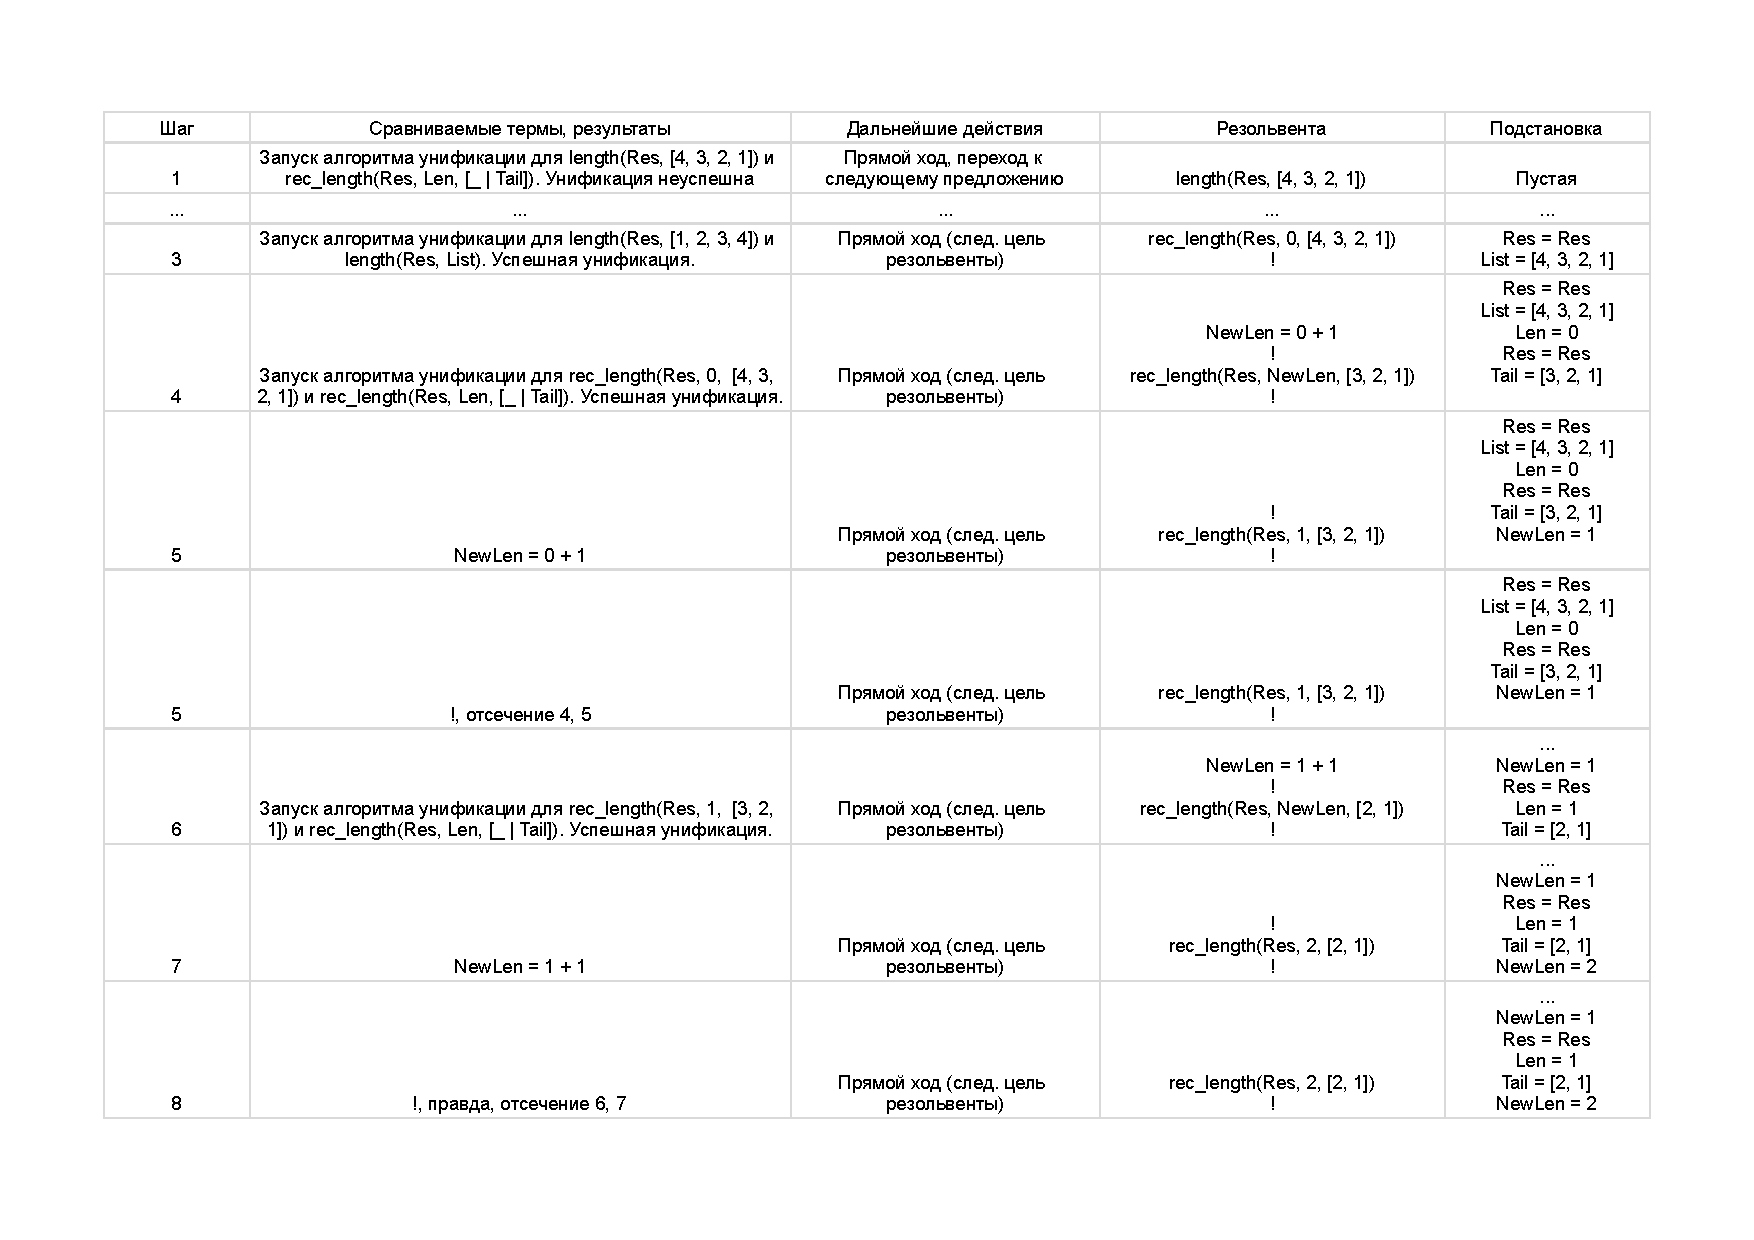
\includegraphics[scale=0.7]{imgs/table_17-1.pdf}
	\end{center}
\end{figure}
\vspace{-1.65cm}
\begin{figure}[H]
	\begin{center}
		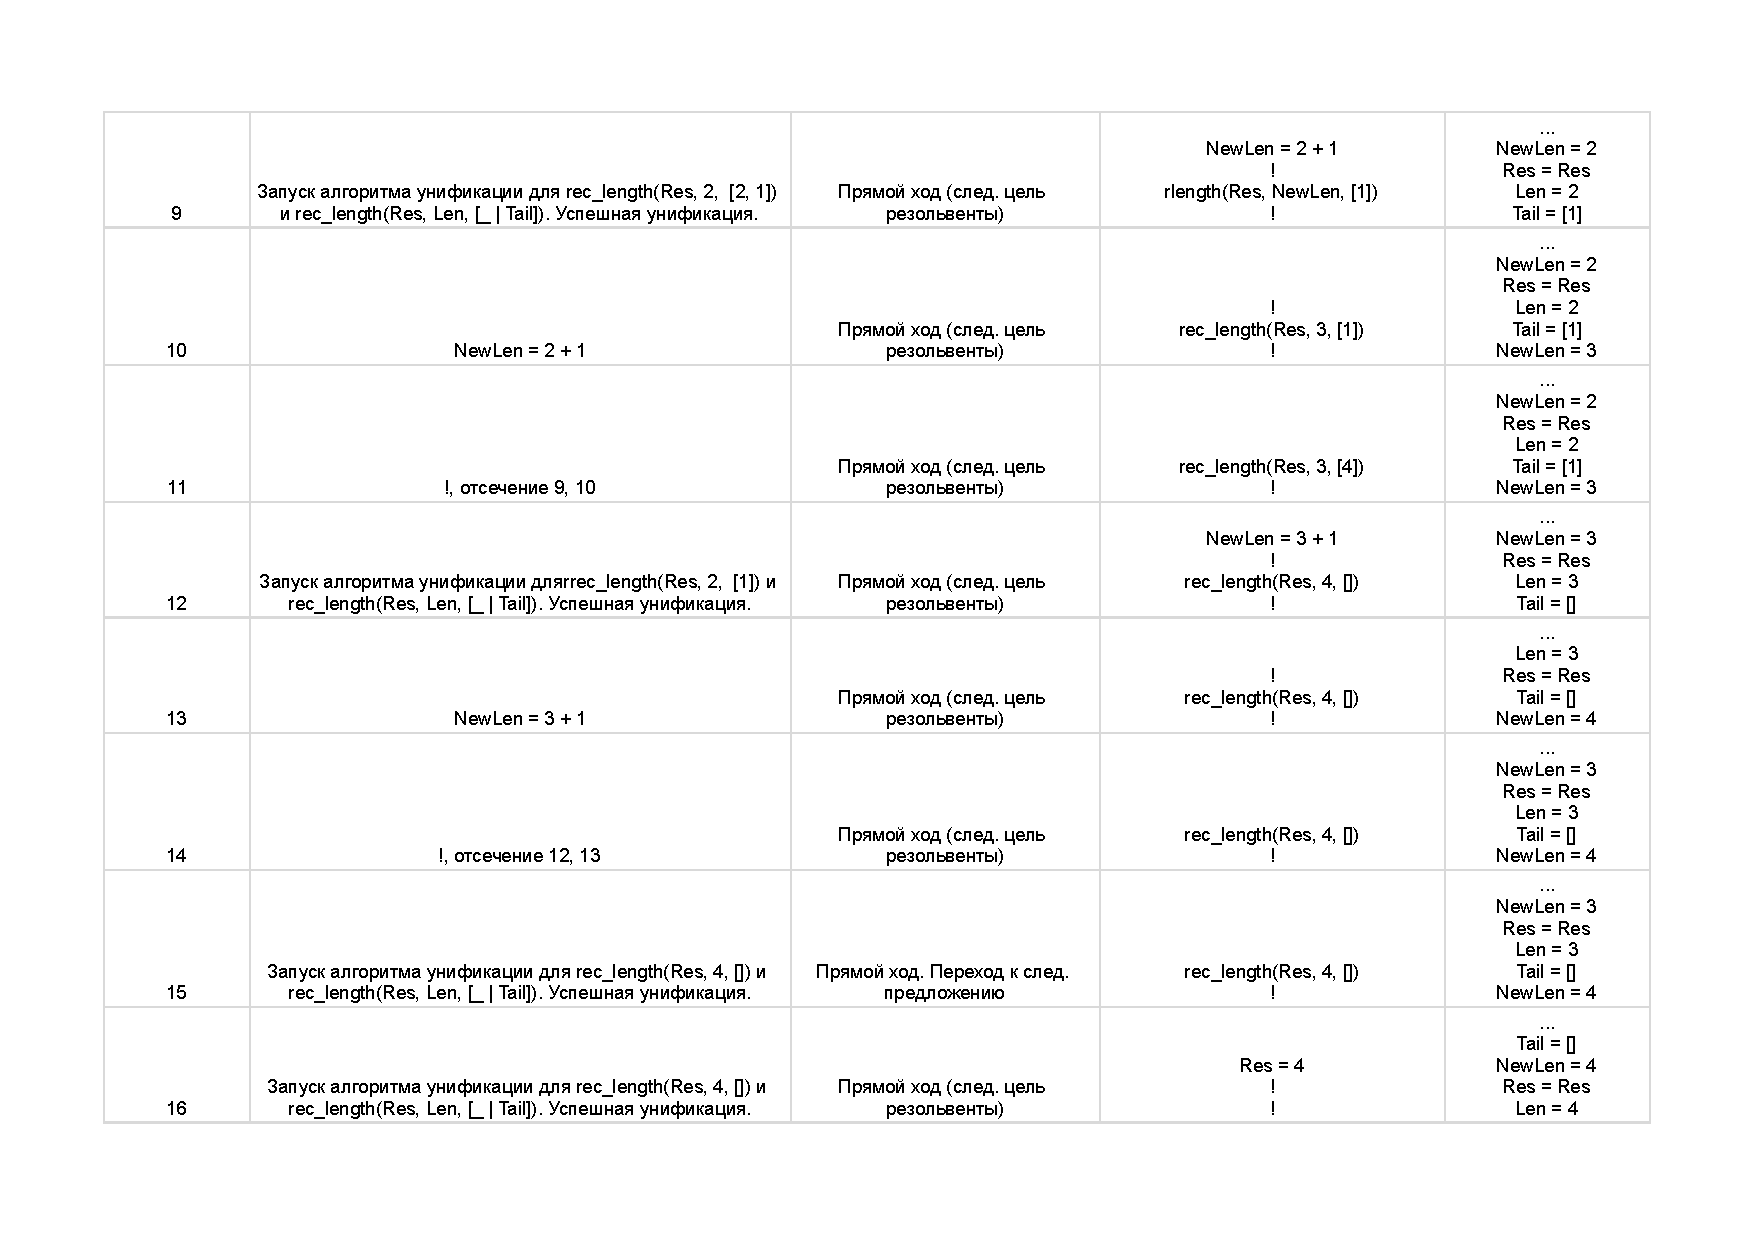
\includegraphics[scale=0.7]{imgs/table_17-2.pdf}
	\end{center}
\end{figure}
\vspace{-1.65cm}
\begin{figure}[H]
	\begin{center}
		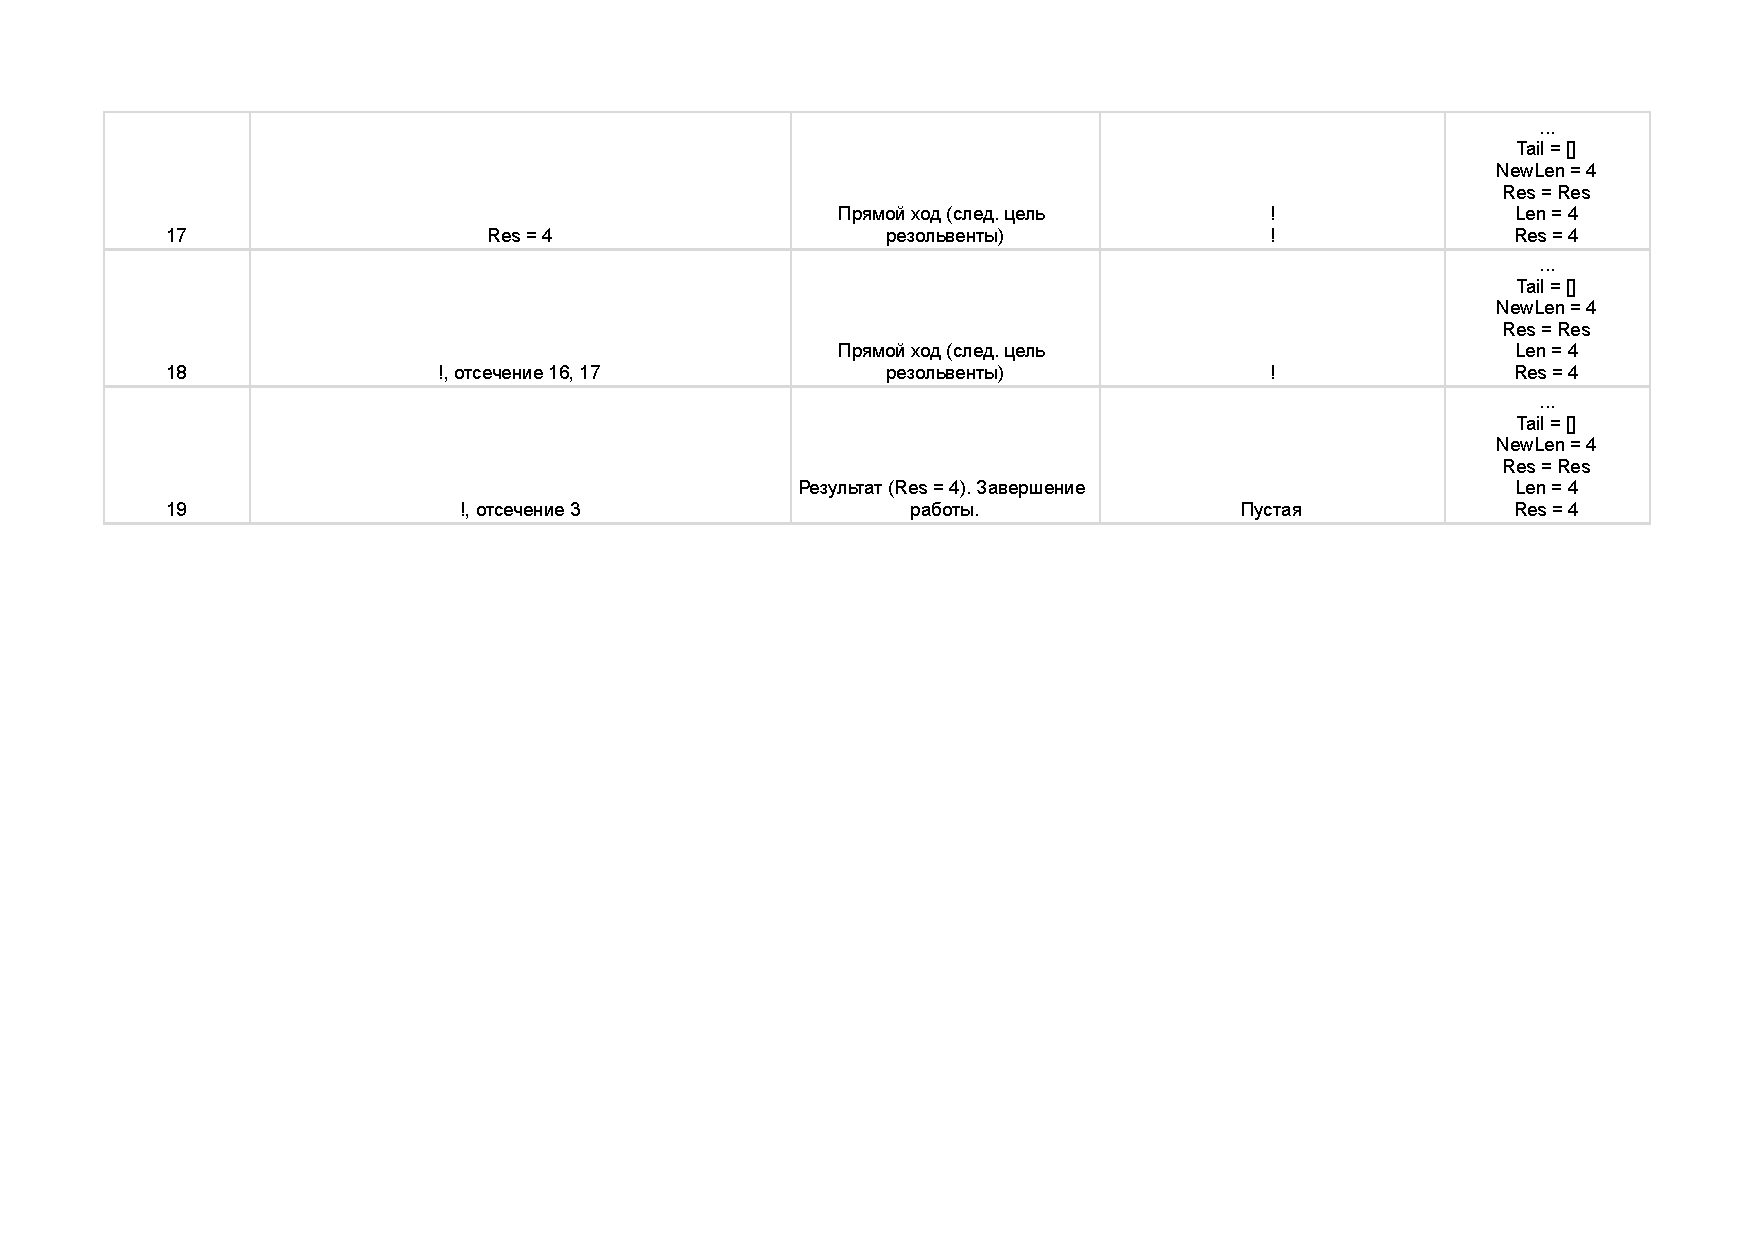
\includegraphics[scale=0.7]{imgs/table_17-3.pdf}
	\end{center}
\end{figure}

\chapter*{Лабораторная работа №18}

\section*{Задание}

Используя хвостовую рекурсию, разработать, комментируя аргументы, эффективную программу, позволяющую:

\begin{enumerate}
	\item Сформировать список из элементов числового списка, больших заданного значения;
	\item Сформировать список из элементов, стоящих на нечетных позициях исходного списка (нумерация от 0):
	\item Удалить заданный элемент из списка (один или все вхождения);
	\item Преобразовать список в множество (можно использовать ранее разработанные процедуры).
\end{enumerate}

Для одного из вариантов ВОПРОСА и 1-ого задания составить таблицу, отражающую конкретный порядок работы системы.

\newpage
\section*{Решение}

\begin{lstlisting}[language=prolog]
domains
	intlist = integer*

predicates
	bigger_than(intlist, integer, intlist)
	odd_list(intlist, intlist)
	single_del(intlist, integer, intlist)
	full_del(intlist, integer, intlist)
	set(intlist, intlist)

clauses
	bigger_than([Head | Tail], N, [Head | ResTail]) :- Head > N, !, bigger_than(Tail, N, ResTail).
	bigger_than([_ | Tail], N, Result) :- bigger_than(Tail, N, Result).
	bigger_than([], _, []).
	
	odd_list([_, Head | Tail], [Head | ResTail]) :- !, odd_list(Tail, ResTail).
	odd_list([], []).
	
	single_del([Head | Tail], N, Tail) :- Head = N, !.
	single_del([Head | Tail], N, [Head | ResTail]) :- single_del(Tail, N, ResTail), !.
	single_del([], _, []).
	
	full_del([Head | Tail], N, [Head | ResTail]) :- Head <> N, !, full_del(Tail, N, ResTail).
	full_del([_ | Tail], N, Result) :- full_del(Tail, N, Result), !.
	full_del([], _, []).
	
	set([Head | Tail], [Head | Result]) :- full_del(Tail, Head, Nt), !, set(Nt, Result).
	set([], []).

goal
	bigger_than([1, 7, 3, 4, 5, 6], 3, Result).
	odd_list([1, 2, 3, 4, 5, 6, 7, 8], Result).
	
	single_del([1, 2, 3, 1, 2, 3, 1, 2, 3], 1, Result).
	full_del([1, 2, 3, 1, 2, 3, 1, 2, 3], 1, Result).
	
	set([1, 2, 3, 1, 2, 3, 1, 2, 3], Result).
\end{lstlisting}

\section*{Порядок работы}

\begin{figure}[H]
	\begin{center}
		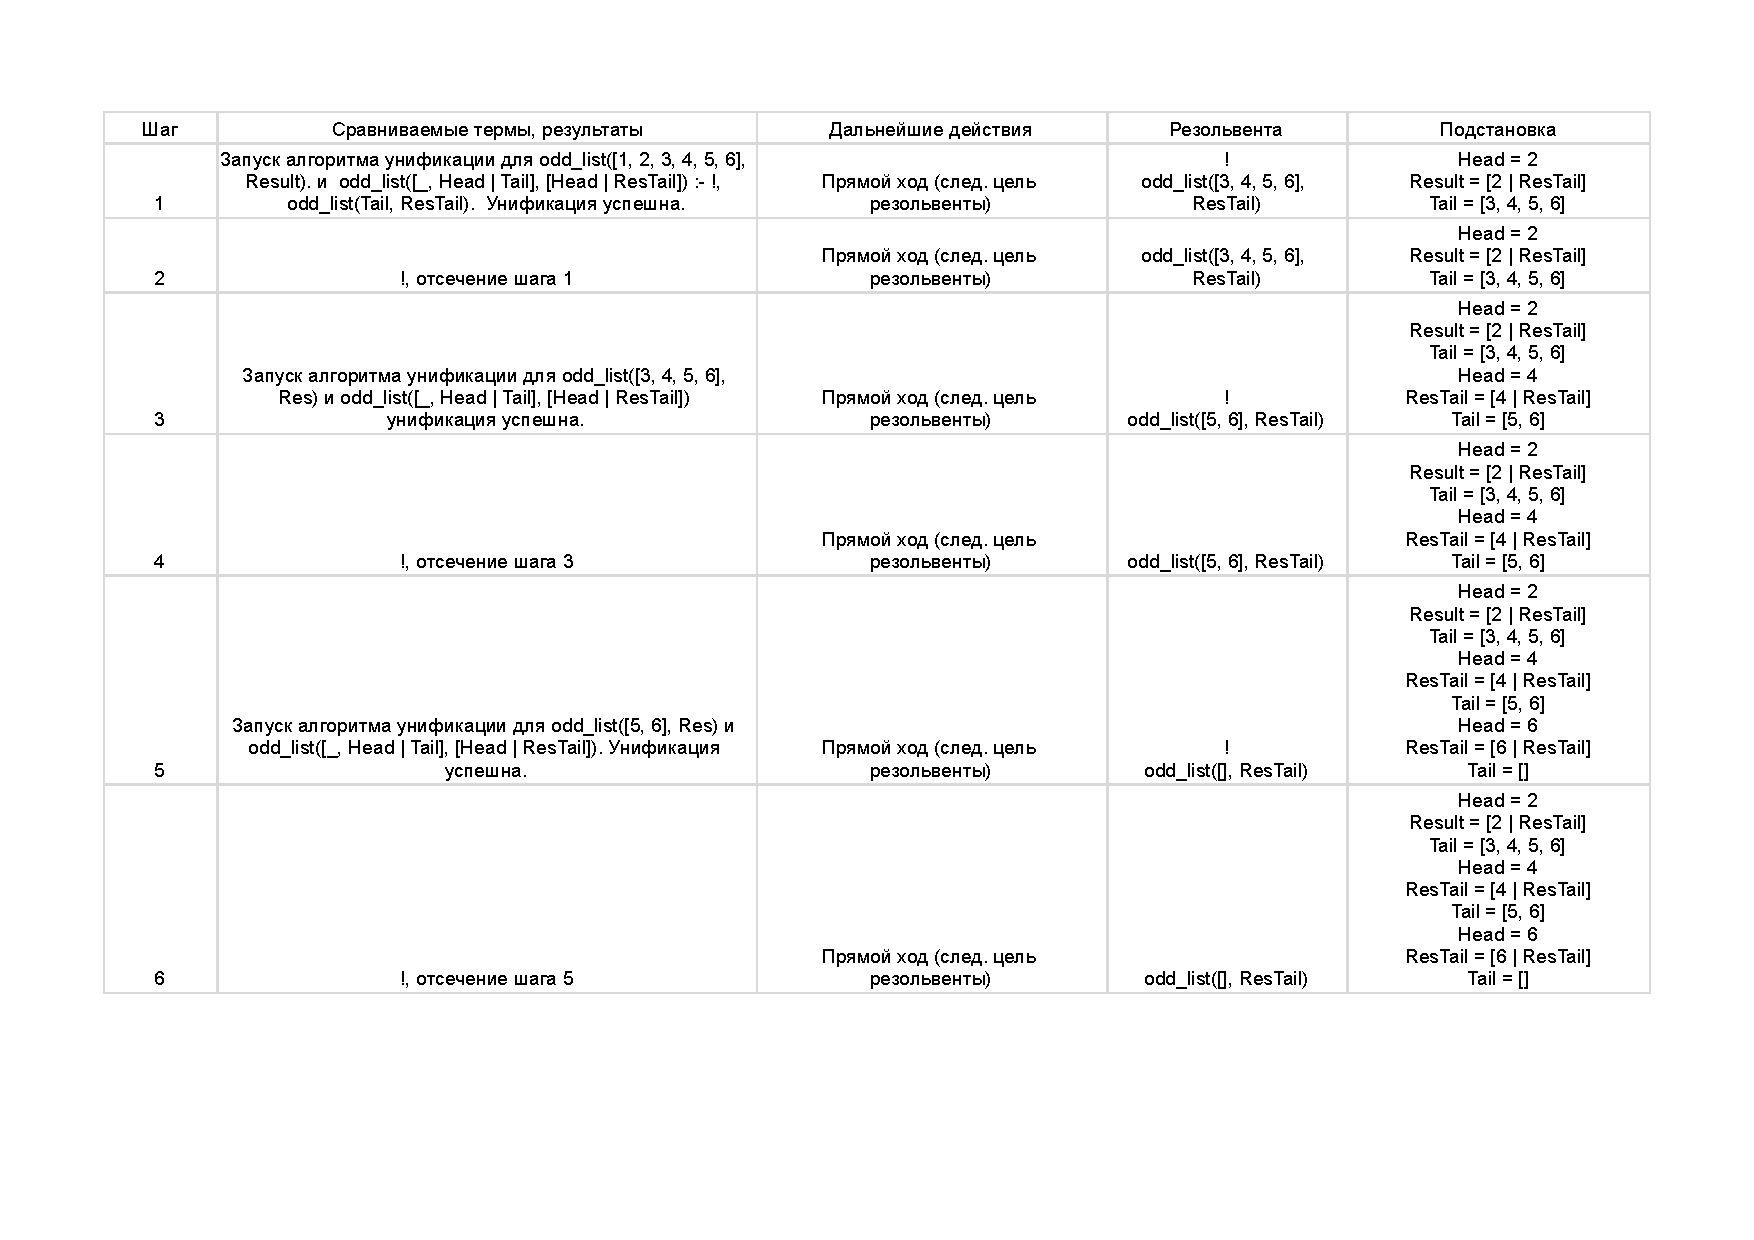
\includegraphics[scale=0.7]{imgs/table_18-1.pdf}
	\end{center}
\end{figure}
\vspace{-1.65cm}
\begin{figure}[H]
	\begin{center}
		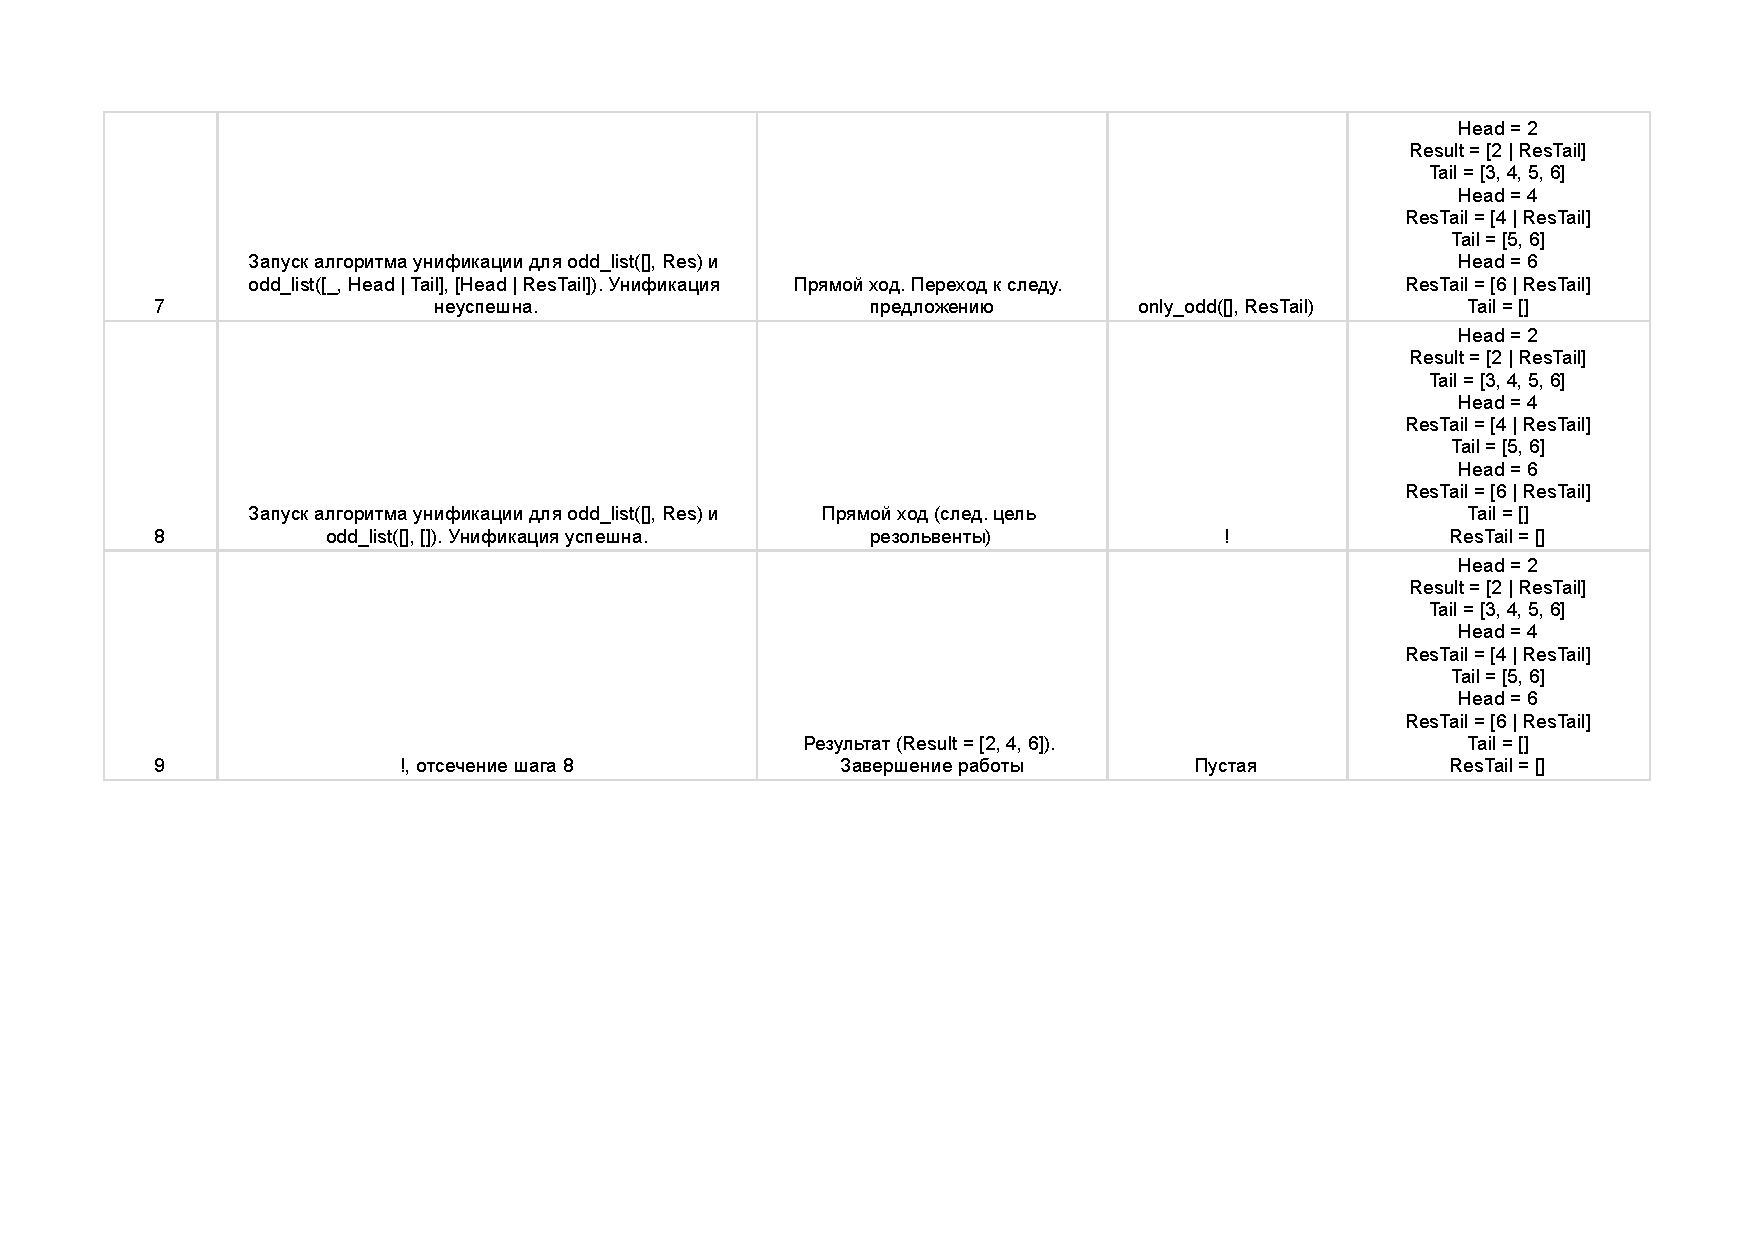
\includegraphics[scale=0.7]{imgs/table_18-2.pdf}
	\end{center}
\end{figure}

\end{document}